\documentclass[twoside]{article}

\usepackage{epsfig}
\usepackage{amssymb}
\usepackage{amsmath}
\usepackage{subcaption}

\setlength{\oddsidemargin}{0.25 in}
\setlength{\evensidemargin}{-0.25 in}
\setlength{\topmargin}{-0.6 in}
\setlength{\textwidth}{6.5 in}
\setlength{\textheight}{8.5 in}
\setlength{\headsep}{0.75 in}
\setlength{\parindent}{0 in}
\setlength{\parskip}{0.1 in}

\newtheorem{thm}{Theorem}[section]
\newtheorem{Defn}{Definition}[section]

\newcommand{\lecture}[3]{
   \pagestyle{myheadings}
   \thispagestyle{plain}
   \newpage
   \setcounter{page}{1}
   \noindent
   \begin{center}
   \framebox{
      \vbox{\vspace{2mm}
    \hbox to 6.28in { {\bf  ~Probabilistic Graphical Models 10-708 Notes with Koller and Friedman Textbook\hfill} }
       \vspace{6mm}
       \hbox to 6.28in { {\Large \hfill #1  \hfill} }
       \vspace{6mm}
       \hbox to 6.28in { {\it Lecturer: #2 \hfill Scribes: #3} }
      \vspace{2mm}}
   }
   \end{center}
   \markboth{#1}{#1}
   \vspace*{4mm}
}

\begin{document}

\lecture{3 : Representation of Undirected GMs}{Eric P. Xing}{Xing JunJie} % Lecture name, Lecturer, Scribes

\section{Review}

There are several important concepts and theorems introduced in last lecture about Directed Graphical Models.

\begin{itemize}
\item Local independence: \(For\ each\ variable\ X_i: (X_i \perp NonDescendant_{X_i} | Pa_{x_i}).\) Indicate that in a directed graph, each variable is independent to its nondescendants given its parent.
\item Global independence: \(I(G) = \{(\mathbf{X}\perp{\mathbf{Y}}\ |\ \mathbf{Z})\ :\ d\textrm{-}sep_G(\mathbf{X} ; \mathbf{Y} \ |\ \mathbf{Z})\}.\)The \emph{global} independence is given by d-seperation. Note that there is no need to consider too much about \emph{global and local} things, you can call them whatever you want.
\item A fully connected DAG \(\mathcal{G}\) is an I-map of \emph{any} distribution, since \(I_{l}(\mathcal{G}) = \emptyset \subset I(P)\) for any \(P\).
\item Minimal I-map: A DAG \(\mathcal{G}\) is a minimal I-map of \(P\), if the removal of even a single edge from \(\mathcal{G}\) renders it not an I-map.
\item A distribution may have several I-maps.
\item P-map: A DAG \(\mathcal{G}\) is a perfect map (p-map) of a distribution \(P\) if \(I(P)=I(\mathcal{G})\)
\end{itemize}

Note that not every distribution has a perfect map as DAG. Here is an example:
\[A\perp C|\{B,D\}\quad B\perp D|\{A, C\}\]

\begin{figure}[!hb]
\centering
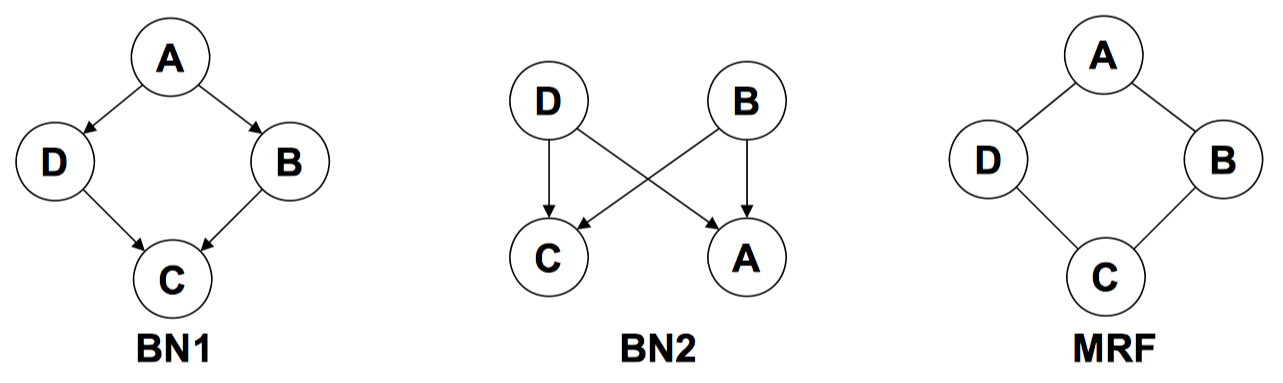
\includegraphics[width=.8\linewidth]{assets/dgm_unable.png}
\caption{\label{fig:dgm_unable} BN1 wrongly says \(B\perp D|A\), BN2 wrongly says \(B\perp{D}\)}
\end{figure}

It is impossible for a DAG to capture both of the two independences at same time. The main reason is that the directed model (sometimes) encodes more independences together with the one we want. Thus, there is a portion of the space of distribution that we cannot encode with a DGM. That motivates another type of graphical model: undirected graphical models, aka Markov Random Fields.

\section{Undirected Graphical Models}

UGMs are very similar to DGMs in structure; but the directed or undirected edges encode differently. The directed model encodes \emph{causal} relationship between nodes, while UGMs captures pairwise relationship which represents \emph{correlation} between nodes, rough affinity.

Many things can be modeled as a UGM, such as a photo---each pixel can be a node, a go game---the grid chessboard seems intuitive, or even social networks, as shown in figure \ref{fig:ugm_ex}.

\begin{figure}[!ht]
\centering
\begin{subfigure}{.3\textwidth}
	\centering
    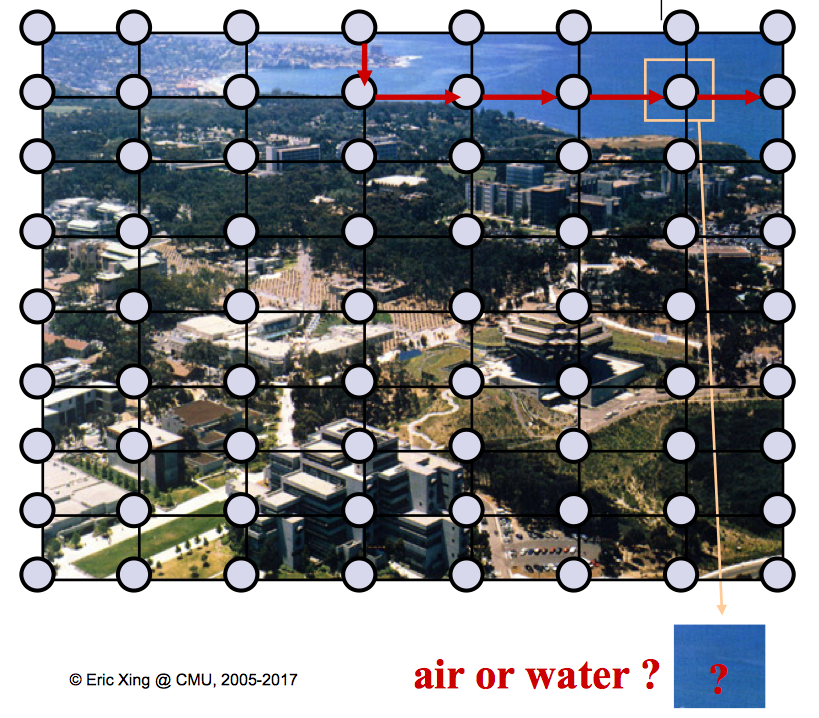
\includegraphics[width=.9\linewidth]{assets/ugm_ex1.png}
    \caption{}
\end{subfigure}
\begin{subfigure}{.3\textwidth}
	\centering
    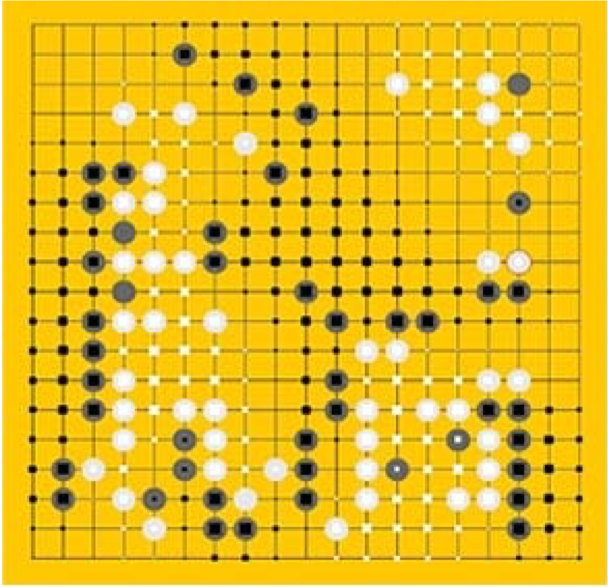
\includegraphics[width=.9\linewidth]{assets/ugm_ex2.png}
    \caption{}
\end{subfigure}
\begin{subfigure}{.3\textwidth}
	\centering
    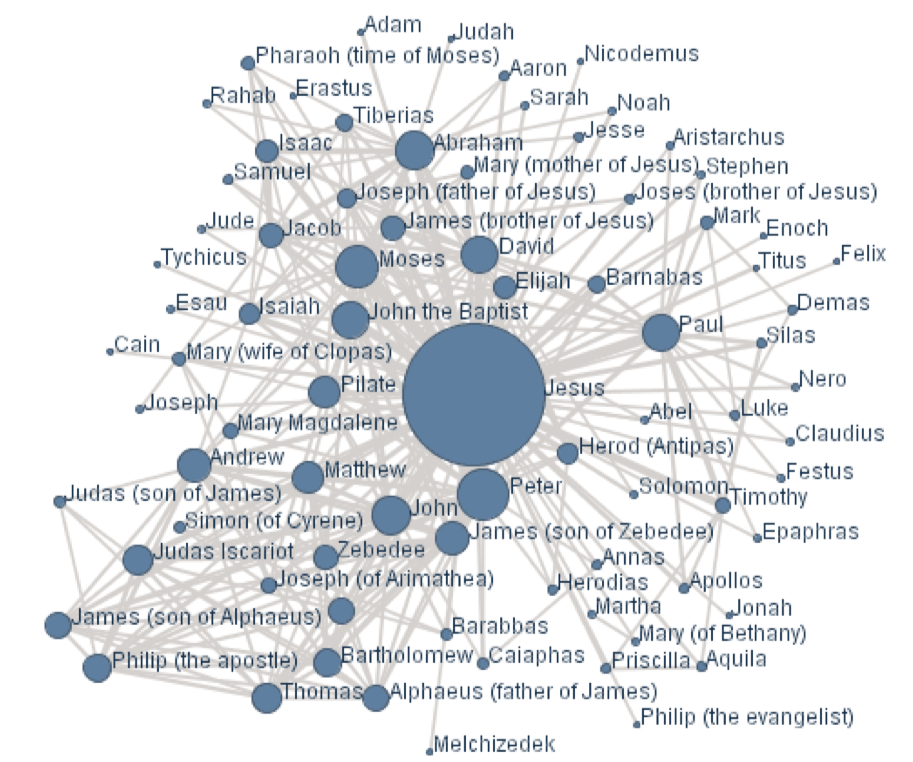
\includegraphics[width=.9\linewidth]{assets/ugm_ex3.png}
    \caption{}
\end{subfigure}
\caption{UGM examples}
\label{fig:ugm_ex}
\end{figure}

\section{Representation}
\begin{Defn}
an undirected graphical model represents a distribution \(P(X_1,\ldots,X_n)\) defined by an undirected graph \(H\), and a set of positive potential functions \(y_c\) associated with the cliques of \(H\), s.t.
\begin{equation}
	P(X_1,\ldots,X_n) = \frac{1}{Z} \prod_{c\in C}{\psi_c(X_c)}
    \label{equation:1}
\end{equation}
where \(Z\) is known as a partition function:
\begin{equation}
	Z = \sum_{X_1, \ldots, X_n} \prod_{c\in C}(\psi_c(X_c))
\end{equation}
\end{Defn}
The potential function can be understood as an contingency function of its arguments assigning ``pre-probabilistic'' score of their joint configuration. We call this of distribution in equation \ref{equation:1} as \textbf{Gibbs distribution}, as \emph{Definition 4.3 in Koller textbook}. And the potential function is defined as \textbf{factor} in Koller textbook.

\begin{Defn}
For \(G={V, E}\), a complete subgraph (clique) is a subgraph \(G'={V'\subseteq {V},E'\subseteq{E}}\) such that nodes in \(V'\) are fully interconnected.A (maximal) clique is a complete subgraph s.t. any superset \(V^{\prime\prime} \supset V'\) is not complete.
\end{Defn}

\subsection{Interpretation of Clique Potentials}

\begin{figure}[!ht]
 \centering
 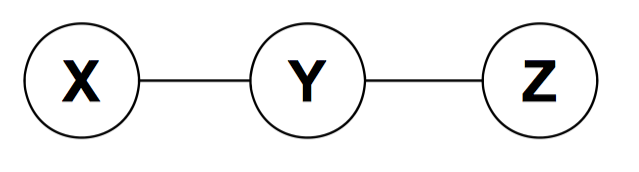
\includegraphics[width=.4\linewidth]{assets/clique_potential.png}
\end{figure}

The model implies \(X\perp Z|Y\). This independence statement implies (by definition) that the joint must factorize as:\[p(x,y,z)=p(y)p(x|y)p(z|y)\]
We can write this as \[p(x,y,z)=p(x,y)p(z|y)\] or \[p(x,y,z)=p(x|y)p(z,y)\]

However, we cannot have all potentials be marginals and cannot have all potentials be conditionals.

The positive clique potentials can only be thought of as general ``compatibility", ``goodness" or ``happiness" functions over their variables, but not as probability distributions.

\subsubsection{Example UGM --- using max cliques}

Here we'll use an example to show an UGM.

\begin{figure}[!h]
	\centering
    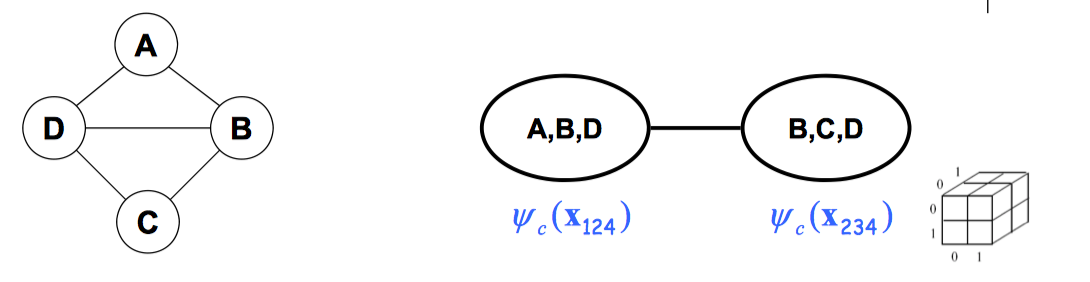
\includegraphics[width=.8\linewidth]{assets/ugm_max_clique.png}
\end{figure}

We can factorize the graph into two max cliques:
\[P(x_1,x_2,x_3,x_4)=\frac{1}{Z}\psi_c(X_{123})\times \psi_c(X_{234})\]
\[Z=\sum_{x_1,x_2,x_3,x_4}\psi_c(X_{123})\times \psi_c(X_{234})\]

We can represent \(P(X_{1:4})\) as two 3D tables instead of one 4D table.

\subsubsection{Using subcliques}

In this example, the distribution factorized over the subcliques.

\begin{figure}[!h]
	\centering
    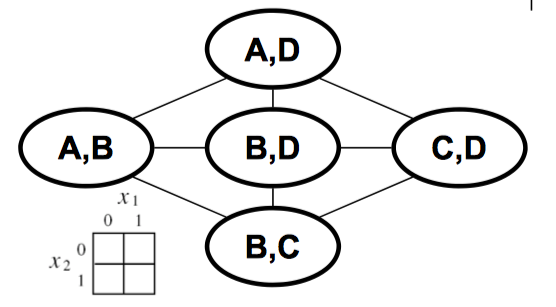
\includegraphics[width=.4\linewidth]{assets/ugm_sub_clique.png}
\end{figure}

\[
\begin{split}
P(x_1,x_2,x_3,x_4) & = \frac{1}{Z}\prod_{ij}\psi_{ij}(X_{ij}) \\
& = \frac{1}{Z}\psi_{12}(X_{12})\psi_{14}(X_{14})\psi_{23}(X_{23})\psi_{24}(X_{24})\psi_{34}(X_{34}) \\
Z & = \sum_{x_1,x_2,x_3,x_4}\prod_{ij}\psi_{ij}(X_{ij})
\end{split}
\]

\subsubsection{Example UGM --- canonical representation}

A canonical representation of such a graph can be expressed as:

\[
\begin{split}
P(x_1,x_2,x_3,x_4) & = \frac{1}{Z}\psi_c(X_{123})\times \psi_c(X_{234}) \\
& \times \frac{1}{Z}\psi_{12}(X_{12})\psi_{14}(X_{14})\psi_{23}(X_{23})\psi_{24}(X_{24})\psi_{34}(X_{34}) \\
& \times \psi_{x_1}(x_1)\psi_{x_2}(x_2)\psi_{x_3}(x_3)\psi_{x_4}(x_4) \\
Z & = \sum_{x_1,x_2,x_3,x_4} \ldots
\end{split}
\]

\subsection{Independence properties}

\subsubsection{Global independence}
\begin{Defn}
A set of nodes \(Z\) separates \(X\) and \(Y\) in \(H\), denoted \(sep_H(X : Y |Z)\), if there is no active path between any node \(X \in \mathbf{X}\) and \(Y \in \mathbf{Y}\) given \(\mathbf{Z}\). Global independences associated with \(H\) are defined as:
\begin{equation}
I(H)={(X\perp Y|Z) :sep_H( X :Y|Z)}
\end{equation}
\end{Defn}

\begin{figure}[!htb]
  \centering
  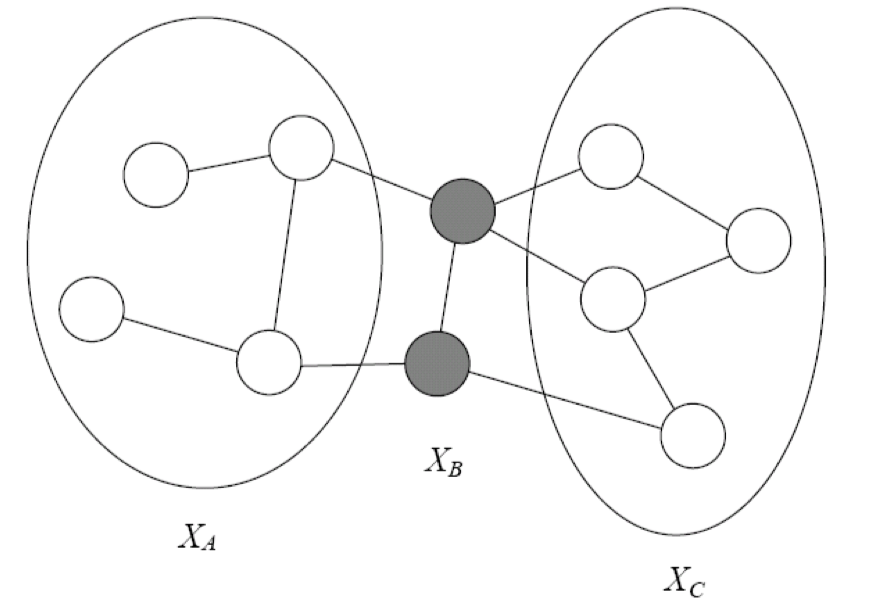
\includegraphics[width=.5\linewidth]{assets/ugm_separate.png}
  \caption{In this, the set \(X_B\) separates \(X_A\) from \(X_C\) . All paths from \(X_A\) to \(X_C\) pass through \(X_B\)}
  \label{fig:separate}
\end{figure}

In Figure \ref{fig:separate}, B separates A and C if every path from a node in A to a node in C passes through a node in B. It is written as sepH(A : C|B). A probability distribution satisfies the global Markov property if for any disjoint A,B,C such that B separates A and C, A is independent of C given B.

\subsubsection{Local independence}

\begin{figure}[!ht]
  \centering
  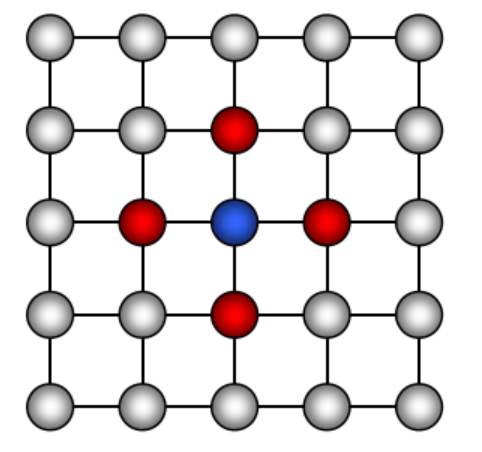
\includegraphics[width=0.4\linewidth]{assets/ugm_local.png}
  \caption{Illustration of Markov Blanket in undirected graph}
\end{figure}

\begin{Defn}
For each node \(X_i \in V\), there is unique Markov blanket of \(X_i\) , denoted \(MB_{X_i}\) , which is the set of neighbors of \(X_i\) in the graph (those that share an edge with \(X_i\) )
\end{Defn}

\begin{Defn}
The local Markov independencies associated with H is:
\begin{equation}
I_l(H): \{X_i \perp V - \{X_i\} - MB_{x_i} | MB_{x_i} : \forall i\}
\end{equation}
\end{Defn}

In other words, X i is independent of the rest of the nodes in the graph given its immediate neighbors.

Note that, based on the local independence:

\begin{equation}
P(X_i|X_{-i}=P(X_i|MB_{x_i})
\end{equation}

\subsubsection{Soundness and completeness of global Markov property}

\begin{Defn}
An UG \(H\) is an I-map for a distribution \(P\) if \(I(H) \subseteq I(P)\), i.e., \(P\) entails \(I(H)\).
\end{Defn}

\begin{Defn}
P is a Gibbs distribution over H if it can be represented as
\begin{equation}
P(X_1, \ldots, X_n) = \frac{1}{Z}\prod_{c\in C}\psi_c(X_c)
\end{equation}
\end{Defn}

\begin{thm}
(soundness): If \(P\) is a Gibbs distribution over \(H\), then \(H\) is an I-map of \(P\).
\end{thm}

\begin{thm}
(Completeness): If X and Y are not separated given Z in H (\(\lnot sep_H (X ; Z |Y )\)), then X and Y are dependent given Z, in some distribution P represented as (\(X \not\perp_P Z|Y \)) that factorizes over H.
\end{thm}

The proof of the theorems are available on Koller textbook.

\subsubsection{Other Markov properties}

For directed graphs, we defined I-maps in terms of local Markov properties, and derived global independence.For undirected graphs, we defined I-maps in terms of global Markov properties, and will now derive local independence.

The pairwise Markov independencies associated with UG H = (V;E) are

\[I_p(H)=\{(X\perp Y|V-\{X,Y\}):{X,Y}\notin E\}\]

\begin{figure}
  \centering
  
\includegraphics[width=.5\linewidth]{assets/ugn_pair_independence.png}
  \caption{Pairwise independence in undirected graph. Red nodes are observed.}
  \label{fig:pairwise_independence}
\end{figure}

For example, in figure \ref{fig:pairwise_independence}, we have the following independence

\[X_1\perp X_5 | \{X_2, X_3,X_4\}\]

\subsubsection{Relationship between local and global Markov properties}

\begin{itemize}
\item For any Markov Network H, and any distribution P, we have that if \(P \models I_l(H)\) then \(P \models I_p(H)\)
\item For any Markov Network H, and any distribution P, we have that if \(P \models I_l(H)\) then \(P \models I_p(H)\)
\item Let P be a positive distribution. If \(P \models I_l(H)\), then \(P \models I_p(H)\)
\end{itemize}

The following three statements are equivalent for a positive distribution P:
\begin{itemize}
\item \(P \models I_l(H)\)
\item \(P \models I_p(H)\)
\item \(P \models I(H)\)
\end{itemize}

Above equivalence relies on the positivity assumption of \(P\). For nonpositive distributions, there are examples of distributions \(P\), there are examples which satisfies one of these properties, but not the stronger property.

\subsubsection{Perfect maps}

\begin{Defn}
A Markov network H is a perfect map for P if for any X; Y;Z we have that
\begin{equation}
sep_H(X;Z|Y) \Leftrightarrow P \models (X\perp Z|Y)
\end{equation}
\end{Defn}

Note that, just like DMs, not every distribution has a perfect map as UGM.

\subsubsection{Exponential Form}

Constraining clique potentials to be positive could be inconvenient (e.g., the interactions between a pair of atoms can be either attractive or repulsive). We represent a clique potential \(\psi_x(X_c)\) in an unconstrained form using a real-value "energy" function \(\psi_x(X_c)\):

\begin{equation}
\psi_c(X_c) = exp\{-\phi_c(X_c)\}
\end{equation}

Thus, this gives the joint distribution an additive structure:

\begin{equation}
P(X)=\frac{1}{Z}exp\{-\sum_{c\in C}\phi_c(X_c)\} = \frac{1}{Z}exp\{-H(X)\}
\end{equation}

where the \(H(X)\) is called the ``free energy''.

The exponential ensures that the distribution is positive. In physics, this is called the ``Boltzmann distribution''.In statistics, this is called a log-linear model (as Koller textbook introduces).

\end{document}